%TC:ignore
\begin{figure}[H]
    \centering
    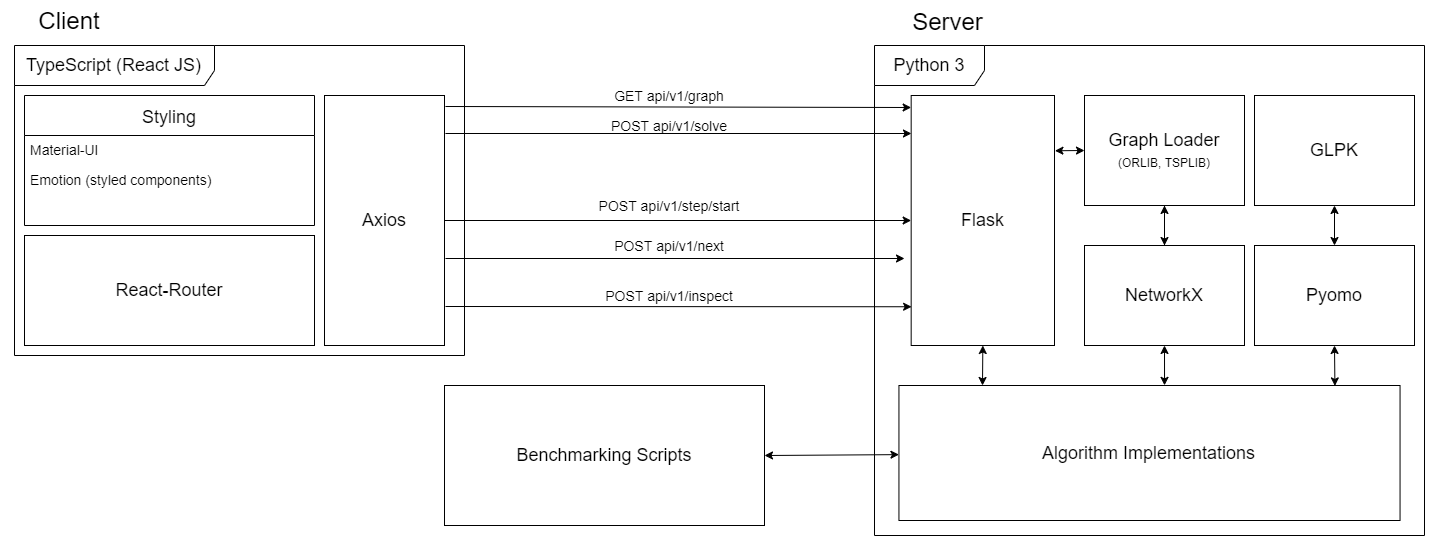
\includegraphics[width=\textwidth]{images/system_architecture.png}
    \caption{System Architecture}
    \label{fig:system_architecture}
\end{figure}
%TC:endignore

\subsubsection{Solution Visualisation (\texorpdfstring{\acrshort{api}}{API} Request)}
The solution visualisation flow contains a single request:
%TC:ignore
\begin{figure}[H]
    \centering
    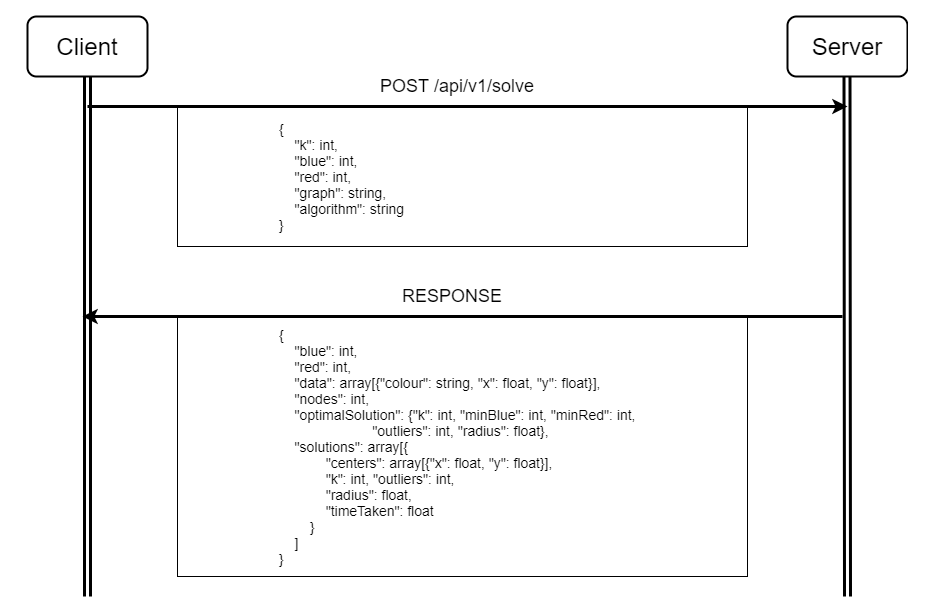
\includegraphics[width=0.85\textwidth]{images/solver_ui/post_solve_flow.png}
    \caption{Solve Request}
    \label{fig:solve_request}
\end{figure}
%TC:endignore

\subsubsection{Stepped Visualisation (\texorpdfstring{\acrshort{api}}{API} Request)}
The stepped solver is a multi request flow; it is initialised through the '/start' endpoint which creates a solver iterator and returns a \acrshort{uuid} token. The solver iterator (response, \cref{fig:stepped_next_inspect_request}) is implemented using a Python generator function which allows us to use lazy evaluation to execute the next step in the algorithm only when needed.
%TC:ignore
\begin{figure}[H]
    \centering
    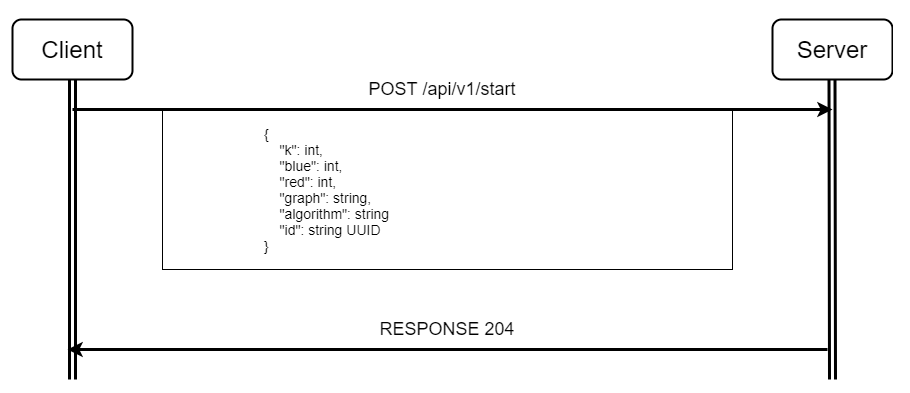
\includegraphics[width=0.8\textwidth]{images/stepped_solver_ui/start_stepped_flow.png}
    \caption{/api/v1/start flow}
    \label{fig:stepped_start_request}
\end{figure}
%TC:endignore

Subsequent calls to the '/next' and '/inspect' endpoints with the UUID is used to exhaust the iterator. Inspect moves to the next chronological step and next skips to the next major step.
%TC:ignore
\begin{figure}[H]
    \centering
    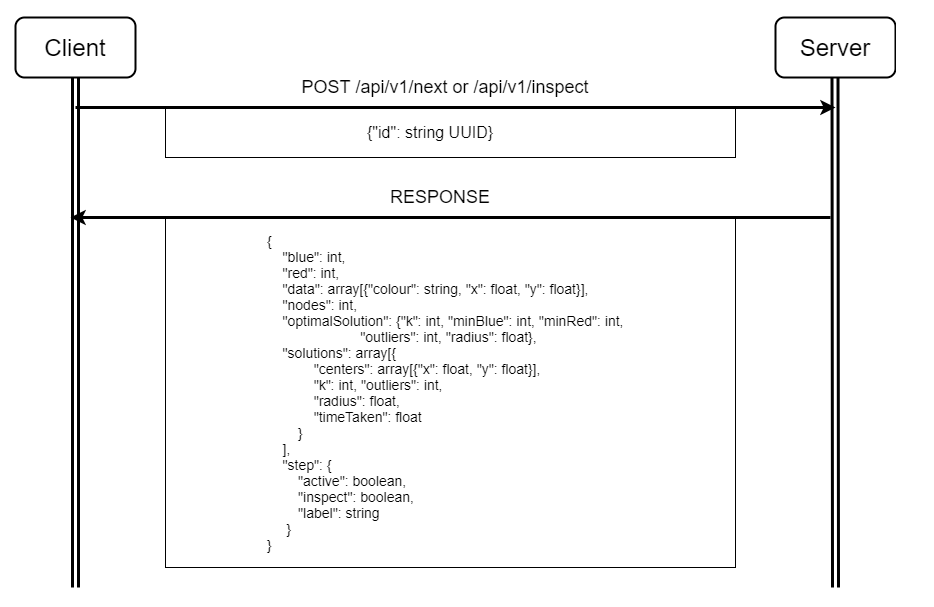
\includegraphics[width=0.8\textwidth]{images/stepped_solver_ui/next_inspect_stepped_flow.png}
    \caption{/api/v1/next and /api/v1/inspect flow}
    \label{fig:stepped_next_inspect_request}
\end{figure}
%TC:endignore

%\subsubsection{Build and Deployment}
%Following the accessibility requirement, we also consider the ease of setup. As we use linear program solvers, this is an extra dependency that is not installable the dependency manager Python pip. Therefore we use Docker, we configure the build file to create and package the static web files, install all dependencies; a user can clone our git repository, execute 'docker build' and 'docker run', then have a working instance of our application. This also allows us to easily deploy to cloud platforms such as Heroku.